\chapter{Introduction}

\section[Introduction]{\textbf{Introduction}}
As society grows more complex, government faces a challenge and an opportunity. 
The challenge is to deliver on its mission to provide, protect, and prosper in 
an increasingly multifaceted society where it is difficult to develop one-size-fits-all 
programs that meet the precise needs of citizens

To deliver improved services to citizens,
governments at every level are faced with similar
set of challenges. One example is how to harness
the big data which has been acquired through
various touch points and other sources in order
to deliver impactful and relevant services along
with generating meaningful insights for intelligent
decision making.

As government delivers on its timeless mission to
provide for its citizens, protect them, and help
them prosper, it delivers services across a value
chain. That begins with reform, moves through
operations, delivers a service, measures
outcomes, and then begins again.

By adopting an artificial intelligence and machine
learning aligned data-driven strategy,
government can see the benefits of digital
transformation. Such a transformation can help
you to design innovative new business models. 
across multiple channels, optimize processes,
engage citizens and partners more effectively,
and manage change successfully. Armed with
360-degree insight, real-time recommendations,
and greater agility, you can better see the root
cause of problems, look for viable solutions, and
deploy them quickly. It can also help you to
report critical outcomes internally and externally,
reduce improper payments, and develop more
meaningful and impactful public policy. In short,
the transformation can help you function more
efficiently while increasing public trust and
support.




% You are allowed to use figures or diagrams which can help in introducing the topic acknowledging the source. For example , if you are introducing a particular topic, an appropriate figure can be used. The figure should be referenced in the text as Figure. \ref{fig:universe} 
\noindent\makebox[\textwidth]{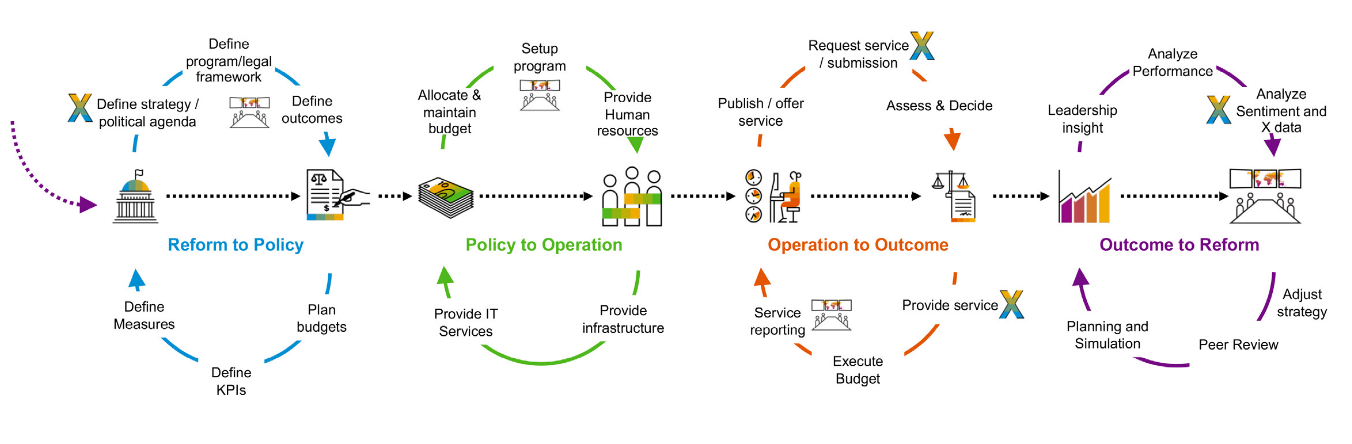
\includegraphics[width=\paperwidth]{Chapter1/Figures/img1.png}}
% \begin{figure}[htb]
% \centering
% 	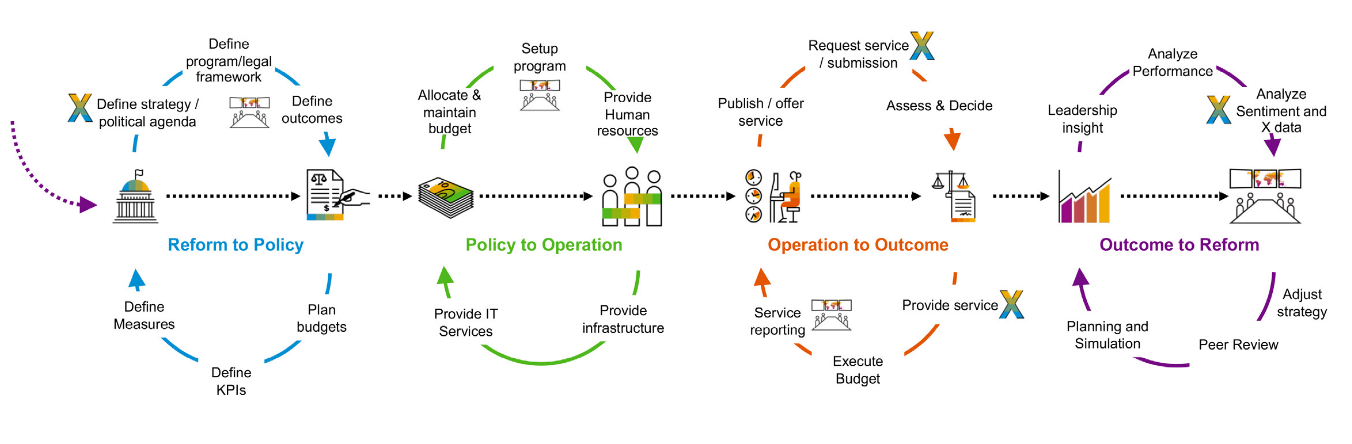
\includegraphics[width=\paperwidth]{Chapter1/Figures/img1.png}	
% 	\caption{Sample picture of universe }
% 	\label{fig:universe}
% \end{figure}

% These guidelines are provided to formally expose you to the various ethical and technical issues involved in writing up your work and the format you are required to adhere to while submitting your project report.


\section[Purpose]{\textbf{Purpose}}
The study’s goal is to provide a enterprise solution with several functions of most public sector related
governance and operations such as budget planning, expense tracking, and grant management all at once. The technologies are intended to effectively map real information to
aid clients in going live by aiding in client creativity along with client assistance.




\section[Motivation]{\textbf{Motivation}}
The methods that government typically uses to
evaluate policies and outcomes may no longer be
sufficient to calibrate needed programs. As
complexity rises, the world is becoming more
interdisciplinary - problems can and do have
multiple root causes. The inability to approach
these root causes from multiple perspectives can
limit the efficacy of government action to solve
them.

However, most governments are not similarly managing
their data as a strategic asset to solve citizen problems,
meet citizen needs, and better understand the
consequences of potential new policies. Government
organizations still largely consider money, people,
facilities, and systems (not necessarily data) as their chief
assets. Very often data is perceived more as a problem
than a strategic asset.

% Brief the motivation of selecting your project title. You can elaborate the challenges in the specific area, relevance and importance of the chosen topic. 

\section[Problem statement]{\textbf{Problem statement}}

The core mission of the public sector – to protect the community, provide services,
and help the economy prosper – remains firmly in place. For public organizations,
success is measured not only by financial return on investment but even more so by
political and social return. Changes in technologies, citizen expectations, operational
models, and standards themselves require constant adaptation. Public sector
organizations must be able to respond to rapidly changing conditions and continue to
deliver outcomes within budget, yet still comply with standards

Designed to help all levels of government maximize public value, SAP for Public Sector solutions enable governments to optimize limited resources in public administration while delivering responsive front-office services. Our solutions support business processes across a wide range of government functions, from accounting and procurement to case management and social services.

SAP solutions help governments leverage their finite time, money, and personnel resources to fulfill mandated program and service requirements on a timely basis. Where two or more agencies share responsibility for a common outcome, these solutions can integrate information, processes, and technology to support the active collaboration that delivers financial returns, as well as social and political results, to internal and external government stakeholders. 

\section[Objectives]{\textbf{Objectives}}
This digital age is disruptive. Public sector organizations need strategic priorities that drive transformation. SAP envisions reimagined end-to-end (E2E)
business scenarios to support the strategic priorities of the digital economy.

The objectives of the project are
\begin{enumerate}
\item Put the citizen at the center

Continue your journey by further simplifying complicated
processes for the citizen, providing personalized, self-managed,
secure online engagement. Deliver the best customer experience
by connecting the front office to the back office. Become
anticipatory service orchestrators, information brokers, and
networkers.
\item Reimagine business processes and models

Lay a digital foundation for more efficient and agile processes,
to be able to quickly change when unforeseen disruptions
occur. Proactively adapt operational models and augment
everyday tasks so government workers can focus on the cases
that require human engagement.

\item Leverage data as an asset

Create a culture that is open and transparent – one that values
evidence over intuition and is based on an organization-wide
“single source of truth” that integrates interorganizational and
external data. Prioritize protection of data and privacy. Improve
services to citizens by adopting a data-driven strategy that
enables action from insight.

\item Enable the workforce of the future

Give employees every opportunity to do and be their best. Align
employee skills with organization needs, reduce compliance risk,
and keep remote workers engaged and productive. Track and
manage employee health and assess workforce engagement
and well-being. Understand potential implications for culture,
productivity, and the organization overall
\end{enumerate}

\section[Scope and relevance]{\textbf{Scope and relevance}}
Organization in public sector manage fund, budget and grants from multiple sources.
Allocation and consumption of funds are based on the needs of the organization.
Proper tracking and analysis of funds is key to effective management of funds.
Utilizing data driven approach helps in keeping track of available funds and their usage 
to better plan expenses and predict the requirements.  


\section[Literature Survey]{\textbf{Literature Survey}}
% https://www.sap.com/documents/2017/01/a4303fdd-a07c-0010-82c7-eda71af511fa.html
% https://help.sap.com/doc/367477e6c8b94385bcd6404f06bc4c86/1.0.0.3/en-US/SBP_10FP03_Application_Help_en.pdf

% A literature review is a text of a scholarly paper, which includes the current knowledge including substantive findings, as well as theoretical and methodological contributions to a particular topic. Literature reviews are secondary sources, and do not report new or original experimental work. Most often associated with academic-oriented literature, such reviews are found in academic journals, and are not to be confused with book reviews that may also appear in the same publication. Literature reviews are a basis for research in nearly every academic field . A narrow-scope literature review may be included as part of a peer-reviewed journal article presenting new research, serving to situate the current study within the body of the relevant literature and to provide context for the reader. In such a case, the review usually precedes the methodology and results sections of the work.

\subsection{ERP Systems in Public Sector}

The vast majority of ERP system implementation in
production systems has been completed and consequently
the needs of that market have been satisfied. Some other
potential areas of ERP systems implementation were in
focus of ERP systems manufacturers. One of the emerging
markets is the public sector. Implementation of ERP
systems in the public sector has already began regardless
of some well-known ERP implementation problems such
as enormous investment and risk of failure in
implementation itself. Numerous published scientific
papers deal with various aspects of ERP systems, but the
number of papers regarding ERP systems implementation
in the public sector is relatively small. That particular area
of the public sector is becoming increasingly interesting for
ERP systems manufacturers, and researchers are interested
in the areas of public services where the ERP systems have
already been implemented. \cite*[]{Robert2014}

Following are the feilds where the ERP system can be systematically incorporated in Public sector 

\begin{table}[H]
    \fontsize{10}{12}\selectfont
    \caption{Public Sector}
    \label{c1:tab1}
    \begin{center}
    \begin{tabular}{|p{3cm}|c|c|c|}
        %\hline
        %\multicolumn{4}{|c|}{Country List} \\
        \hline
        \textbf{Code }& \textbf {Non economic public sector} \\ \hline
        \textbf{PS1}    &   Education       \\\hline
        \textbf{PS2}    &   Culture         \\\hline
        \textbf{PS3}    &   Health careful  \\\hline
        \textbf{PS4}    &   Social Services \\\hline
        \textbf{PS5}    &   Law Enforcement \\\hline
        \textbf{PS6}    &   Military – defense\\\hline
        \textbf{PS7}    &   Public library   \\\hline
    \end{tabular}
    \end{center}
    \end{table}
    


\subsection{Available ERP Solutions}

\subsubsection*{Aptean}

Aptean was founded in 2012 after a merger between Consola Corporation and CDC Software and currently offers ERP solutions for several financial and manufacturing markets. The company builds and acquires solutions to support the evolving operational needs of businesses. Aptean’s ERP solutions include Cimnet ERP, Encomprix ERP, Ross ERP, and more, each designed to fit individual needs. Aptean delivers solutions to global customers in the manufacturing, distribution, high tech, transportation, retail, government, real estate, financial services, health care, and not-for-profit industries. \cite{Budget2019}


\subsubsection*{Deltek}

Deltek’s ERP solution, Costpoint, has assisted companies in researching and identifying new opportunities, winning new business, recruiting and developing talent, and more. Deltek offers a range of ERP products to fit the unique demands of clients. Deltek’s ERP solutions are available as cloud-based and on-premise systems, priced per employee per month. Deltek is typically used by organizations with over 21 employees and more than ten users who need the software. The solution is used in several industries, including aerospace and defense, healthcare, non-profits, and education.  \cite{Nizar2021}


\subsubsection*{Infor}
Infor is a privately held software company founded in 2002. Infor’s business applications are specialized by industry, built for the cloud, and gives you everything you need to run your day-to-day operations as well as grow your business for the long term. Whether you need to optimize vital back-office functions like HR and financials, jumpstart your customer experience, or initiate digital transformation, Infor solutions have you covered. Over 90,000 organizations worldwide rely on Infor to help overcome market disruptions and achieve business-wide digital transformation.
\cite{Rachel2022}


\subsubsection*{Microsoft}
Microsoft provides ERP software to businesses of all sizes through its Dynamics 365 platform, consisting of six products: Microsoft AX, GP, SL, NAV, CRM, RMS. The Microsoft Dynamics portfolio started in 2001 with the acquisition of Great Plains Software and Soloman and in 2002 with the acquisition of Navison and Axapta. Together, these four technologies make up the Microsoft Business Solutions Group (MBS), a major supplier of ERP solutions. Dynamics GP, NAV, and SL are typically intended for small and medium enterprises, while Dynamics AX is best suited for larger organizations.

\cite{Robert2014}


\subsubsection*{Oracle NetSuite}
For more than 20 years, Oracle NetSuite has helped organizations grow, scale, and adapt to change. NetSuite provides a suite of cloud-based applications, including financials / ERP, HR, professional services automation, and omnichannel commerce, used by more than 15,000 customers in 203 countries and dependent territories. ERP software from Oracle NetSuite allows consolidation in real-time and includes automated intercompany eliminations and foreign currency translation. The solution is web-based and runs on a range of Internet browsers. The company ensures safety by using its built-in security controls and data center.

\cite{Thompson2019}


\subsubsection*{OpenGov}
OpenGov provides cloud ERP solutions for public sector budgeting, community development, and financial management. Over 1,000 governments across the U.S. rely on OpenGov to help allocate resources, increase efficiency, improve public engagement, and make data and information readily available to staff and elected officials. The OpenGov ERP Cloud offers four main products: Budgeting and Planning; Financials; Reporting and Transparency; Permitting, Licensing and Code Enforcement.
\cite{Vasyl2021}

\subsubsection*{SAP}
SAP, the German software giant, provides businesses with its SAP S/4HANA next-generation ERP software that provides strong functionality across many industries, including manufacturing, services, retail, wholesale distribution, and more. S/4HANA offers applications covering customer relationship management, financials, human capital management, and product lifecycle management. The software primarily serves small to medium-sized businesses with one hundred employees and less than 75 million USD in annual revenue.


\subsubsection*{Tyler Technologies}

Tyler Technologies’ solutions help governments and schools better serve their communities with technology designed to simplify complex processes. This vendor’s broad solutions and product offering empower you to deliver better and faster assistance to the public — greater transparency and accessibility, sustainable office practices, secure data that’s easy to manage and maintain, and faster results. Tyler Technologies offers various solutions geared toward public administration, courts and public safety, health, human services, and K-12 education.

\subsubsection*{Unanet}
Unanet for Government Contractors makes managing GovCon projects easy, providing perfect clarity and total control over day-to-day operations, forecasting, and planning. Purpose-built in-house by GovCon professionals, Unanet features support DCAA requirements at each stage. This vendor also integrations PSA and PPM with Financials to help organizations reliably plan, track, and manage projects and people. Unanet also offers ERP for professional services and A/E.

% \ref{fig:ERPmillitary} 
\begin{figure}[H]
\centering
	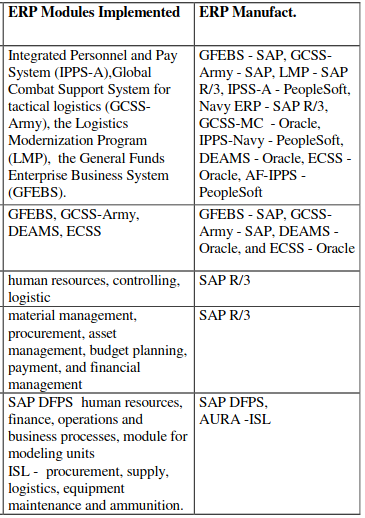
\includegraphics[scale=0.5]{Chapter1/Figures/ERP3.png}	
	\caption{ERP system used in millitary sector} 
	\label{fig:ERPmillitary}
\end{figure}

% \ref{fig:ERPEducation} 
\begin{figure}[H]
\centering
	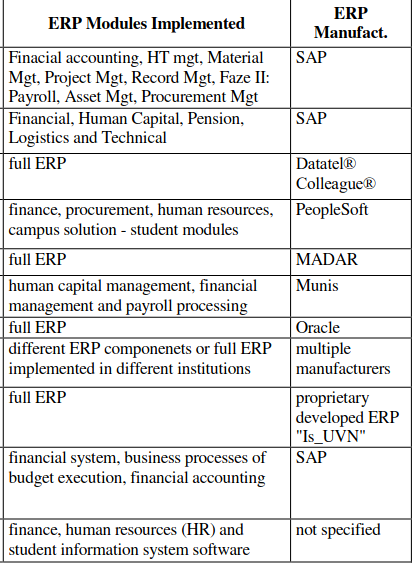
\includegraphics[scale=0.5]{Chapter1/Figures/ERP1.png}	
	\caption{ERP system used in education sector}
	\label{fig:ERPEducation}
\end{figure}

% \ref{fig:ERPFinance} 
\begin{figure}[H]
\centering
	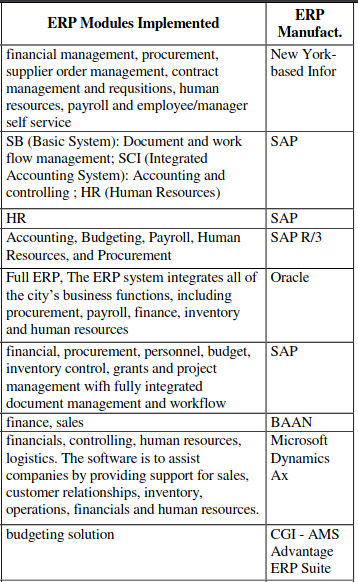
\includegraphics[scale=0.5]{Chapter1/Figures/ERP2.png}	
	\caption{ERP system used in financial sector }
	\label{fig:ERPFinance}
\end{figure}

% \ref{fig:ERPHealthcare} 
\begin{figure}[H]
    \centering
        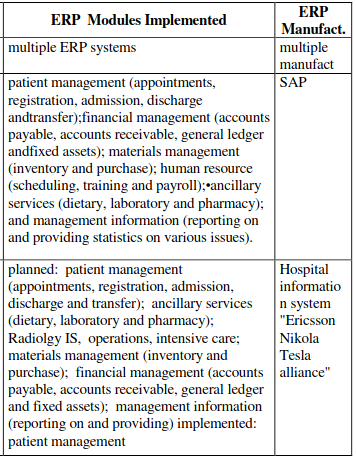
\includegraphics[scale=0.5]{Chapter1/Figures/ERP4.png}	
        \caption{ERP system used in healthcare sector }
        \label{fig:ERPHealthcare}
    \end{figure}
    

    \section[Methodology and Architechtural Roadmap]{\textbf{Methodology and Architechtural Roadmap}}
    % Discuss about the methodology you identified to execute the objectives of your project in brief. Methodology is a system of practices, techniques, procedures, and rules used to execute a particular project. You can elaborate the methodology in a later chapter. Here you can present in the form of a flow diagram and explain the methodology in a paragraph.
    The steps adopted during the implementation of the Budget Planning Application can
    be shown as a three stage pipeline as discussed below :
    
    \begin{itemize}
    \item Use of SAP UI5 and SAP Fiori for the deployment of the front-end system. A glimpse
     of the Fiori LaunchPad is shown in the diagram below. It shows the catalogue
     containing a suite of applications customized according to user preferences and
     packages.
     
    \begin{figure}[H]
        \centering
            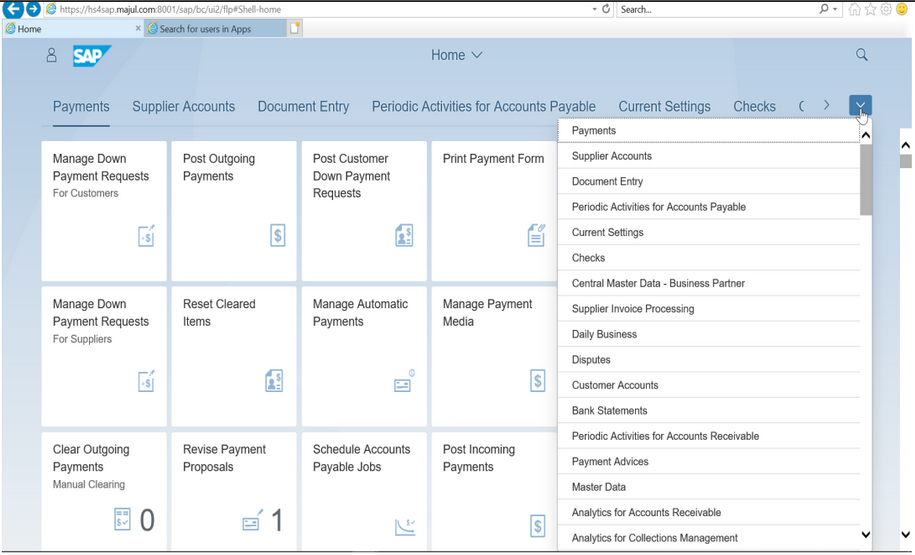
\includegraphics[scale=0.5]{Chapter1/Figures/fiori1.png}	
            \caption{Fiori LaunchPad} 
            \label{fig:fiorilaunchpad}
    \end{figure}
        
    \item Setting up SAP S/4 HANA databases for collecting and capturing info received
        through the programs. The database can analyze significant volume actual statistics
        in a brief period.
    \item Server-side code on the backend built upon SAP ABAP.
    \item  To get an expedient solution for data representation, Core Data Services Views are
        supported by the current relational databases and views.
    \item  SAP NetWeaver Gateway Client and Open data Protocol are used toh link
        backend with frontend resources.
    \end{itemize}
    
        \begin{figure}[H]
            \centering
                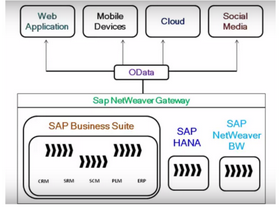
\includegraphics[scale=0.5]{Chapter1/Figures/odata.png}	
                \caption{SAP Odata Protocol} 
                \label{fig:odataprotocol}
        \end{figure}
            
        The figure above shows a high level framework of the different tiers and the connection
        amongst all components. The Odata and Netweaver Gateway are mainly used for the
        interlinking of front-end and backend services.
    
    
        The features to be provided include-
    
        \begin{itemize}
            \item Budget requests, reviews and adoption- Manage budgets in a single application
    
            \item Operating, capital and grants budgeting - A single application for all budget types
    
            \item User configuration - Tailor budget forms, process controls, reports and analytics to your unique budgeting requirements and adapt them to changing requirements
            \item Personnel cost forecasting - Examine and plan personnel expenditures at a highly granular level to support budgeting, spending plans and collective bargaining
            \item Modeling and analytics - Powerful modeling tools combined with the strength of SAP Business Objects for reporting, dashboards and ad hoc analysis
    
    \end{itemize}
    
    
\section{Organization of Report}
The report is organised into seven chapters which are as follows:

{\bf Chapter 1} This section elaborates how the Budget Planning platform features distinctive functions
that may greatly assist public sector finance departments with thousands/even millions of
bank connections including maintaining transaction signatory info.

{\bf Chapter 2} : This section reviews the prerequisites of the aim of the project. The functional
and non-functional specifications for the implementation of the Budget Planner are discussed along
with the software and hardware requirements.

{\bf Chapter 3} : High level diagrams including the UML Class diagram, sequence diagram,
architecture diagram, data flow diagram, etc are discussed in chapter 3 to comprehend the
flow of information.

{\bf Chapter 4} : Its operational specifics, including the norms utilised for code review, are
detailed in this section. Furthermore, basic needs as well as solutions would be explained.

{\bf Chapter 5} : The validation and verification of the various functionalities of the MBA app are
detailed here. Unit testing, Regression testing and Integration testing are elaborated upon.

{\bf Chapter 6 and 7} : Chapter six and seven mainly demonstrate the results and elaborate on the
analysis obtained hence forth. An ultimate conclusion, along with limitations and future
enhancement of the product are also presented.

\section{Summary}
Ultimately, this section illustrates the importance in streamlining financial client relations
throughout the worldwide community. The Budget Planner enables consumers to
oversee the procedure of creating / consuming funds by providing one-stop
management of the lifespan for public sector. This software assists clients in becoming
more self-sufficient by  lowering overall need on every type of assistance.


% \subsubsection[Review types]{\textbf{Review types}}

% The main types of literature reviews are: evaluative, exploratory, and instrumental. A fourth type, the systematic review, is often classified separately, but is essentially a literature review focused on a research question, trying to identify, appraise, select and synthesize all high-quality research evidence and arguments relevant to that question. A meta-analysis is typically a systematic review using statistical methods to effectively combine the data used on all selected studies to produce a more reliable result.


% \subsubsection[Process and product]{\textbf{Process and product}}

% Distinguish between the process of reviewing the literature and a finished work or product known as a literature review. The process of reviewing the literature is often ongoing and informs many aspects of the empirical research project. All of the latest literature should inform a research project. Scholars need to be scanning the literature long after a formal literature review product appears to be completed.

% \subsubsection{\textbf{Page limitation}}

% A careful literature review is usually 15 to 30 pages and could be longer. The process of reviewing the literature requires different kinds of activities and ways of thinking and link the activities of doing a literature review with Benjamin Bloom’s revised taxonomy of the cognitive domain (ways of thinking: remembering, understanding, applying, analysing, evaluating, and creating).

% This section should contain the review of the literature in the past.You should review a minimum of 10 papers from standard reference journals. Kindly avoid local conference papers and papers from predatory journals. Kindly consult with your guide and finalize papers to be considered for review before adding in this section.Report the major observations and findings from each paper in one paragraph in the format given below.

%  proposed various techniques for adders and multipliers.Add the reference papers to the bibliography section using Jabref and cite it here using the instructions given in further chapters.


% \subsubsection{\textbf{Plagiarism}}

% To use someone else's exact words without quotation marks and appropriate credit, or to use the unique ideas of someone else without acknowledgement, is known as plagiarism. In publishing, plagiarism is illegal; in other circumstances, it is, at the least, unethical. You may quote or paraphrase the words or ideas of another if you document your source. Although you need not enclose the paraphrased material in quotation marks, you must document the source. 

% Paraphrased ideas are taken from someone else whether or not the words are identical. Paraphrasing a passage without citing the source is permissible only when the information paraphrased is common knowledge in a field. (Common knowledge refers to historical, scientific, geographical, technical, and other type of information on a topic readily available in handbooks, manuals, atlases and other references). 

% \subsubsection{How to add Reference}
% Use \texttt{Jabref} which will help in adding the reference in a separate file, from which one can use \verb|\citep\{\}| command to add reference. A sample, referring to a textbook would look something like this,\cite{Razavi2000}.

% \cite{Budget2019}
% \cite{Nizar2021}
% \cite{Rachel2022}
% \cite{Robert2014}
% \cite{Thompson2019}
% \cite{Vasyl2021}

% \section[Brief Methodology of the project]{\textbf{Brief Methodology of the project}}
% Discuss about the methodology you identified to execute the objectives of your project in brief. Methodology is a system of practices, techniques, procedures, and rules used to execute a particular project. You can elaborate the methodology in a later chapter. Here you can present in the form of a flow diagram and explain the methodology in a paragraph.

% \section[Assumptions made / Constraints of the project]{\textbf{Assumptions made / Constraints of the project}}

% List the assumptions made for the execution of the project in this section. You can also elaborate on the major constraints of the project. This section should clearly state under what conditions your project is valid. It is mandatory to have this section in your project report.

% \section[Organization of the report]{\textbf{Organization of the report}}

% This report is organized as follows. Write the discussions in each chapter. A sample is as follows.
% \begin{itemize}
% \item Chapter 2 discusses the fundamentals of ADC and the performance parameters for evaluation.
% \item Chapter 3 discusses .
% \item Chapter 4 discusses .
% \item Chapter 5 discusses .
% \item Chapter 6 discusses .
% \end{itemize}

.